%MWH: had to move this here to get it to show up on page 2
\begin{figure*}[t]
\begin{center}
\scalebox{.7}{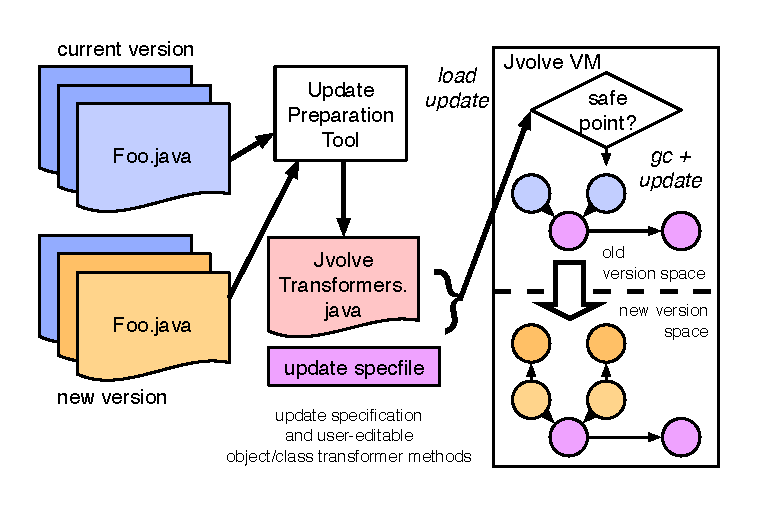
\includegraphics{system}}
\end{center}
\caption{Dynamic Software Updating with \DSU}
\label{fig:overview}
\end{figure*}



\section{Dynamic Updates in \DSU}

This section overviews how \DSU{} performs dynamic updating, including
the sorts of updates that \DSU{} supports, and how the developer
participates in the process.

%%  the developer responsibilities and how \DSU{}
%% performs updates.  We then summarize the simple update model that we
%% currently support.  Although simple, these updates are sufficient for
%% most of our test suite.  We postpone to Section~\ref{sec:saftey} our
%% discussion of the safety and flexibility implications of our simple
%% updates and of unsupported more sophisticated updates because they are
%% best understood once the VM collector and JIT support are explained in
%% Section~\ref{sec:VMdesign}.  Next, we give a running example to
%% help explain some of the issues with a VM based approach. 

\subsection{System Overview}

Figure~\ref{fig:overview} illustrates the dynamic update process.  It
shows the VM running the current version of the program and at top
left, the source files.  Meanwhile, developers are working on a new
version,
% \footnote{ Recent work in refactoring can help users prepare
%   their updates~\cite{HD:05}}
whose source files are shown at the
bottom left.  When the new version is ready--it compiles correctly and
the developer has fully tested it using standard procedures---the
developer passes the old and new versions of the source tree to \DSU's
\emph{change detector}.  This tool identifies classes that have
been added or changed and copies them into a separate directory.

At this point, the developer may write some number of \emph{object}
and \emph{class transformers}.
Transformer methods take an object or class of the old version and
produce an object or class of the new version.  For example, if an
update to class \texttt{Foo} adds a new instance field \texttt{x} and
a new \texttt{static} field \texttt{y}, the programmer can write an
object transformer (called \texttt{jvolve\_object}) to initialize
\texttt{x} for each updated object, and a class transformer (called
\texttt{jvolve\_class}) to initialize \texttt{y}.  If the programmer
chooses not to write one of these transformers, the system will
dynamically produce a default one that simply initializes each new field to its
default value and copies over the values of any old fields that have
not changed type.  Transformer methods are the only portions of code
where both views of the class definition are visible and they are only
ever invoked at update time.  This feature enables the programmer to
develop the application largely oblivious to the fact that it will be
dynamically updated.

%% The user compiles $v_1$ with \textsf{javac}, or
%% another Java to bytecode compiler, which guarantees that the update is
%% free from type, syntactic, and other errors.  For example, if the
%% update modifies a method signature, the update is guaranteed to
%% contain the updated versions of any class file that invokes the
%% method.

\DSU{} then translates the transformer functions to class files, which
ensures (among other things) that they are type correct.  The running
VM then starts the updating process by loading the transformers and the new
user class files.
% The first step is for the VM's JIT compiler to
% compile the loaded classes. 
  Next, the VM waits for all the threads to
stop at a DSU \emph{safe point}~\cite{HicksNettles03,neamtiu06dsu}
where none of their activation stack's
contain \emph{updated methods}. Updated methods include all the
directly updated methods and any methods that depend on them or
updated classes, e.g., due to inlining. Section~\ref{sec:safe}
describes some additional restrictions on safe points.  

The VM then adds any new entries to the method dispatch table, 
and invalidates any updated method implementations.  Changed methods
are then compiled as 
a matter of course the next time the program invokes them (and the old
implementations can never be accessed).  Finally,
the VM initiates a full copying garbage collection to update the state
of existing objects whose classes changed.  When the collector
encounters an object to update in the \emph{from space}, it allocates a copy
of this object and an object of the new class in the \emph{to space}. At the
end of the collection, \DSU{} runs object transformers on
each of these pairs and then invokes the class transformers.
At this point, the update is complete.

% Taken from outline.txt
% Section 2: Updating model (look at Dynamic ML paper section 2 for guidance)
%  Workflow
%    Show picture of the process
%      Develop patches
%      Compile them, ensure type correctness
%      Load 'em via classloading
%      Wait for the threads to reach a safe point, stop them, run GC
%        Intuitively discuss safe point condition; elaborate later
%      restart and resume (now the new version)

\subsection{Update Model}
\label{sec:updates}

We have designed a
flexible, yet simple update model that supports updates that we
believe are important in practice.  \DSU{} classifies updates into the
following two categories:

\begin{description}

\item[Method body updates:] These updates change just the internal
implementation of a method.
  
\item[Class updates:] These updates change the class signature by adding
or removing fields and methods, or by changing the signature of fields and
methods in a class.

\end{description}

\noindent 
Method body updates are the simplest and most commonly supported
updates~\cite{JVMhotswap,VSEnC,eaddy05enc,GilmoreKW97,orso:java,K42reconfig,HjalmtyssonG98},
because these changes do not require DSU safe points; they can be
applied at any time and preserve type safety.
Permitting only method implementation updates however prevents many
common changes~\cite{neamtiu05evolution}.  For example,
Section~\ref{sec:experience} shows that over half of the updates to
Jetty, JavaEmailServer and CrossFTP add fields and/or change
method signatures.

\begin{figure*}[t]
\begin{tabular}{c|c}
\begin{minipage}{3in}
\begin{footnotesize}
\begin{verbatim}
public class User {
  private String username, domain, password;
  private String[] forwardAddresses;
  public String[]
   getForwardedAddresses() {...}
  public void
   setForwardedAddresses(String[] f) {...}
}
public class ConfigurationManager {
  private User loadUser(...) {
     ...
     User user = new User(...);
     String[] f = ...;
     user.setForwardedAddresses(f);
     return user;
  }
}
\end{verbatim}
\end{footnotesize}
\end{minipage} &
\begin{minipage}{3.15in}
\begin{footnotesize}
\begin{verbatim}
public class User {
  private String username, domain, password;
  private EmailAddress[] forwardAddresses;
  public EmailAddress[]
   getForwardedAddresses() {...}
  public void
   setForwardedAddresses(EmailAddress[] f) {...}
}
public class ConfigurationManager {
  private User loadUser(...) {
     ...
     User user = new User(...);
     EmailAddress[] f = ...;
     user.setForwardedAddresses(f);
     return user;
  }
}
\end{verbatim}
\end{footnotesize}
\end{minipage} \\
(a) Version 1.3.1 &
(b) Version 1.3.2 \\
\end{tabular}
\caption{Example changes to JavaEmailServer \texttt{User} and
  \texttt{ConfigurationManager} classes}
\label{fig:email-example}
\end{figure*}


Class updates may occur at any level of the class hierarchy.  For
example, an update that deletes a field from a parent class will
propagate correctly to the class's descendants. Henkel et al.'s recent work in
refactoring ~\cite{Fowler,HD:05} categorizes changes into the following: renamed
types, moved Java elements, moved static members, changed method
signatures, renamed non-virtual methods, renamed virtual methods, renamed
fields, and generalization where occurrences of a type are replaced by a
particular super-type. \DSU{} supports all these changes.
\DSU{} does not support permutations of the class hierarchy, e.g.,
reversing a super-class relationship.  While this update may be desirable
in principle, in practice, it requires sophisticated transformers that can
enforce update ordering constraints. None of the program versions we
observed made this type of update.
% there are two problems.  First, it may be quite
% challenging to actually implement this change---the process of
% transforming old objects from the old to the new class hierarchy is
% complex.  Second, complex changes make it harder to reason that an
% update's semantics will be correct.  To see why, consider that a
% common limitation of existing code updating systems is that they
% support only method body updates, not method signature
% updates~\cite{JVMhotswap,VSEnC,eaddy05enc,GilmoreKW97,orso:java,K42reconfig,HjalmtyssonG98}.
% The reason is that such changes can take effect at any time and
% preserve type safety, whereas changes to method signatures must take
% timing into account.  However, permitting only method implementation
% updates prevents many common changes~\cite{neamtiu05evolution}
% including the example in Figure~\ref{fig:email-example}.  Therefore,
% any practical system must trade off flexibility with
% availability---the more flexible the update, the greater burden on the
% system to ensure that updates are well-timed.
\DSU's update model is quite flexible.  Developers may change a method
implementation to fix a bug.  Developers may enhance functionality by
adding and acting on a new parameter to a method, or by adding a new
field and its access methods to a class (and its subclasses, as desired).
% \DSU's supported updates also match common refactorings, such
% as dividing a method into multiple methods, renaming a class or
% interface, changing types, and renaming fields~\cite{Fowler}.
% Sections~\ref{sec:safe} and~\ref{sec:xformers} provide additional
% details on the safety, flexibility, and implementation of our
% update model and possible enhancements.
Currently, \DSU{} does not
allow classes with such changes as described above to have active methods
on stack when performing the update. We propose to extend \acf{OSR},
as described in section~\ref{sec:safe} can help remove this restriction.

\paragraph{Example.} 
Consider the following update from JavaEmailServer, a simple SMTP and
POP e-mail server.  Figure~\ref{fig:email-example}
illustrates a 
pair of classes that change between versions 1.3.1 and 1.3.2.  These
changes are fully supported by \DSU.  JavaEmailServer uses the class
\texttt{User} to maintain information about e-mail user accounts in the
server.  Moving from version 1.3.1 to 1.3.2, there are two
differences.  First, the method \texttt{loadUser} fixes some problems
with the loading of forwarded addresses from a configuration file
(details not shown).  This change is a simple method update.  Second,
forwarded addresses are represented as an array of instances of a new
class, \texttt{EmailAddress}, rather than \texttt{String}.  This change modifies
the class signature of \texttt{User} since it modifies the type of
\texttt{forwardedAddresses}.  The class's
\texttt{setForwardedAddresses} method is also altered to take an array of
\texttt{EmailAddress}es instead of an array of \texttt{String}s.


\subsection{Class and Object Transformers}
\label{subsec:transformers}

For our example, the \DSU{} change detector  identifies that
the \texttt{User} and \texttt{ConfigurationManager} classes have
changed.  At this point, the programmer may elect to write object
and class transformers or use the defaults.
The user elects to write both a class and object
transformer for the class \texttt{User}, as illustrated in
Figure~\ref{fig:example-xform}.

Object and class transformer methods are simply \texttt{static}
methods that augment the new class.  The class transformer method
\texttt{jvolve\_class} (body not shown) takes no arguments, while the
object transformer method \texttt{jvolve\_object} takes two reference
arguments: \texttt{to}, the uninitialized new version of the object,
and \texttt{from}, the old version of the object.  For both methods,
the old version of the changed class has its version number prepended to its
name.  In our example, the old version of \texttt{User} is redefined as
class \texttt{v\_1\_3\_1\_User}, which is the type of the \texttt{from}
argument to the \texttt{jvolve\_object} method in the new \texttt{User}
class. The \texttt{v\_1\_3\_1\_User} class contains only field definitions
from the original class, defined with access modifier \texttt{public} to
allow them to be accessed from the \texttt{jvolve\_object} method.

The code in transformer methods is essentially a kind of constructor:
it should initialize all of the fields of the new class/object.  Very
often the best choice is to initialize a new field to its default
value (e.g., \texttt{0} for integers or \texttt{null} for references)
or to copy references from the old values.  In the example, the first
few lines simply copy \texttt{username}, \texttt{domain}, and other
fields from their previous values.  A more interesting case is the
field type change to \texttt{forwardedAddresses}. % the user
% initializes the new field by referring to the old field.  The
The
function allocates a new array of \texttt{EmailAddress}es
initialized using the \texttt{String}s from the old array.  Note that
the default transformer function would instead copy the first three
fields as shown, and initialize the \texttt{forwardedAddresses} field
to \texttt{null} because it has changed type.

Supported in its full generality, a transformer method may
reference any object reachable from the global (\texttt{static})
namespace of both the old and new classes, and read or write fields or
call methods on the old version of the object being updated and/or any
objects reachable from it.  \DSU{} presents a more limited interface
similar to that of past work~\cite{ritzau00dynamic,Mala00a}.  In
particular, transformers may only use old objects to initialize new
objects; the only safe access to a new object is through the
\texttt{to} argument.  Transformers may safely copy the contents of
\texttt{from} fields.  These fields may also be dereferenced if the
update has not changed their class, or if it has, after
the referenced objects are transformed to conform to the new class
definition.  \suriya{Clarify the next sentence} At the moment this is achieved by invoking a VM function,
but ultimately we plan to provide more automatic support.
Finally, object transformers may not call methods
on the old object. For example in Figure~\ref{fig:example-xform},
class \texttt{v\_1\_3\_1\_User} is defined in terms of the fields it
contains, \suriya{clarify} while the methods have been removed.  As explained in
Section~\ref{sec:xformers}, these limitations stem from a goal to keep
our garbage collector-based traversal safe and relatively simple.
This interface is sufficient to handle all of the updates we tested, but
other programs may require a more flexible approach. \suriya{so? is this
true?}

\begin{figure}
\begin{small}
\begin{verbatim}
public class v_1_3_1_User {
  public String username, domain, password;
  public String[] forwardAddresses;
}
public class User {
 ...
 public static void jvolve_class() { ... }
 public static void 
  jvolve_object(User to, v_1_3_1_User from) {
    to.username = from.username;
    to.domain = from.domain;
    to.password = from.password;
    // default transformer would have:
    //   to.forwardAddresses = null
    int l = from.forwardAddresses.length;
    to.forwardAddresses = new EmailAddress[l];
    for (int i = 0; i < l; i++) {
      to.forwardAddresses[i] = 
       new EmailAddress(from.forwardAddresses[i]);
}}}
\end{verbatim}
\end{small}
\caption{Example \texttt{User} object transformer}
\label{fig:example-xform}
\end{figure}

If a programmer does not write an object transformer, the VM % merely
initializes new or changed fields to their default values and copies the
values from unchanged fields. \DSU{}'s \ac{UPT} (described in
Section~\ref{sec:prep}) generates
\suriya{inconsistent with the first sentence of
section~\ref{subsec:transformers}}
default versions of the \texttt{jvolve\_object} and
\texttt{jvolve\_class} methods in the same way, which the user may
modify.


%% will have been verified to be type-correct by the Java-to-bytecode
%% compiler. In addition, \DSU{} has to appropriately handle
%% \verb|ConfigurationManager.loadUser|. \suriya{Should we say, we do not allow
%%   it to be on stack}.

%    Show the parts that change
%    Show the state transformer you would write

%  What is the API for the programmer?
%    Off-line patch tool to figure out what methods changed, etc.
%      (programmer doesn't have to worry about this)
%    State transformer as a method of the new class
%      - but only called during the update process
%      - namespace set up to be clear about which object versions
%        you are referring to




%% \subsubsection{Update Form}


%% To allow dynamic updates, \DSU{} must handle these two important types
%% of updates. (a) Changes within a body of a method that do not change
%% the class definitions type system. (b) Changes to the type system,
%% such as addition of fields, and method signatures.

%% (a) After an update, existing code must call the updated version of a
%% method. \DSU{} accomplishes this trivially by using the capabilities of the
%% JVM to recompile the method with its updated version. \DSU{} updates the
%% function indirection tables (the JTOC for static methods and TIB for
%% virtual methods) to point to the new version. This is similar to what
%% happens with JIT compilation of a method.

%% (b) A type T changes as a result of changes to its fields, or method
%% signatures. \DSU{} enforces \emph{representation consistency}
%% \cite{Stoyle-POPL-2005} in which all objects of type T must logically be of
%% type T's latest version. (This is almost copied from Ginseng. What should
%% we do?)

%% \DSU{} supports representation consistency by ensuring that when type T is
%% updated, all objects of that type in the running program are updated to
%% correspond to the new version. For each object of type T, \DSU{} calls a
%% state transformation function $c_{T_{n->n+1}}$ that converts an object
%% $o_T$ of type $T_n$ to one of type $T_{n+1}$. The type transformation
%% function is generated trivially for most updates, by comparing the old and
%% new definitions of a type.

